\section{Introduction}

Quantum computing presents significant potential for addressing computational problems that remain intractable for classical computers, including molecular simulations, optimization problems, and integer factorization~\cite{shor1997,wecker-reactions,cao2018potential,gidney2025factor2048bitrsa}. These computational advantages derive from quantum computers' ability to leverage quantum mechanical phenomena---like superposition, entanglement, and interference---to process information in fundamentally different ways from classical systems. Current research reports that fully functional quantum computers could significantly outperform classical supercomputers for specific computational tasks~\cite{resourceestimation-beverland2022assessing,arute2019quantum,kim2023evidence,morvan2024phase}.

Quantum algorithms are very different from classical algorithms. They require instructions that explicitly utilize quantum mechanical principles to achieve computational advantages. Nonetheless, several principles from classical programming remain valuable in quantum contexts:

\begin{itemize}
\item Standardized instruction sets enables targeting different hardware architectures
\item Dynamic memory allocation optimizes physical qubit usage
\item Automatic error correction mitigates the inherently error-prone nature of quantum operations
\end{itemize}

Quantum error correction, in particular, has been a primary motivation for this work. Unlike with classical error correction, quantum states cannot be directly observed without destroying their quantum properties. Error detection must occur through indirect measurements, with classical feedback mechanisms triggering appropriate quantum corrections~\cite{shor1995scheme}. This requirement transforms what might initially be conceived as ``pure'' quantum programs into hybrid systems that necessarily combine quantum and classical instructions.

Furthermore, quantum operations exist within a Hilbert space, theoretically allowing for infinite possible operations. In practice, a finite universal instruction set approximates any quantum operation to arbitrary precision. Implementing certain gates in this universal set, particularly through techniques like T-gate injection, requires classical measurements to determine whether quantum state corrections are necessary~\cite{bravyi2005universal}.

These considerations highlight a fundamental characteristic of practical quantum computing: quantum programs must frequently be transformed into hybrid programs that interleave classical and quantum instructions to achieve reliable operation. While there has been significant prior work on hybrid quantum-classical languages, existing approaches have primarily focused on developing unified languages that integrate both paradigms within a single programming model. The specific challenge of handling this hybrid nature through transformations across different levels of abstraction—rather than within a single unified language—represents an important gap in the research landscape.

The central research question addressed in this paper is: How can we design a quantum programming framework that seamlessly integrates classical and quantum components, particularly for error correction protocols, while maintaining program semantics and supporting hardware-agnostic compilation? Our objective is a paradigm that empowers developers to express sophisticated quantum algorithms that can be injected with proper error handling at multiple abstraction levels.

\subsection{Current Approaches to Quantum Programming}

Quantum programs have traditionally been shaped by the Quantum Random Access Machine (QRAM) computational model~\cite{knill2022conventions}, in which a classical processor accesses a quantum memory composed of a fixed set of qubits and applies a well-defined set of operations: preparing qubits, applying unitary transformations, and performing measurements. Essentially, classical programs create and dispatch quantum instructions to a quantum processor. This approach, while intuitive from a classical programming perspective, creates substantial challenges when implementing error correction protocols or adaptive quantum algorithms where classical feedback must be tightly integrated with quantum operations.

The QRAM model is certainly universal, capable of implementing any quantum algorithm or error-correction scheme. But just as a classical assembly language is universal, that does not mean it provides any natural structures for common idioms and approaches. 
Our approach retains the QRAM approach of sending instructions to a quantum computer, but 
we believe our stack-based and callback-based approach provides a more modular and natural fit especially when translating among quantum instructions and implementing error-correction schemes. 

\subsection{Our Contribution: The qstack Approach}

We introduce \textbf{qstack}, a quantum programming framework that implements an alternative coprocessor model with a reversed emphasis: quantum programs are structured as sequences of instructions executed by a quantum processing unit (QPU) with access to classical processing capabilities during execution. A key innovation is our treatment of classical components as opaque callbacks within the quantum program; the quantum execution remains primary while classical computation is encapsulated as "black boxes."  This opacity enables qstack to be agnostic about which classical language is used or how complex the classical processing might be. This classical component enables dynamic adjustments, such as state corrections or conditional branches, based on measurement outcomes obtained during runtime. qstack significantly simplifies the compilation process into lower-level operations that naturally interleave classical and quantum instructions.

To make this approach concrete, consider a toy example that demonstrates a repeat-until-success algorithm where a quantum program continues until a desired measurement outcome is achieved.
The program allocates two qubits and prepares them in an entangled (correlated) state. The program measures the first qubit and collects the result, then measures the second qubit and uses that result to determine whether to repeat the computation. This program is expressed in qstack as follows:

\begin{minted}{ruby}
allocate q1:
  allocate q2:
    mix q2
    entangle q2 q1
  measure collect
measure repeat_until_zero
\end{minted}

After the occurrences of the \`{measure} keyword are \`{collect} and \`{repeat\_until\_zero}, which are simply classical functions (implemented in Python) that take one argument, the bit resulting from measuring one qubit (in LIFO order of allocation), and conditionally generate a new quantum computation based on the measurement result. \`{collect} simply stores the bit for later classical use and generates no additional quantum computation, while \`{repeat\_until\_zero} is defined as:\footnote{Also note that for exposition, the main quantum computation is repeated twice, but in practice the initial program could be written as \texttt{repeat\_until\_zero(1)}.}

\begin{minted}{python}
def repeat_until_zero(measurement):
    if measurement == 1:
        return parse_kernel("""
            allocate q1:
              allocate q2:
                mix q2
                entangle q2 q1
              measure collect
            measure repeat_until_zero""")
    else:
        return None
\end{minted}

This simple example illustrates how quantum programs are inherently probabilistic and how qstack handles dynamic control flow. The \texttt{mix} and \texttt{entangle} instructions, defined later, cause the two measurements to either both be 0 or both be 1, with a 50\% chance of either. The collected measurements will be a sequence of 1s terminated by a 0. A histogram of the outcomes shows that the number of outcomes becomes exponentially smaller as the length of the bitstring increases: sequences of length $n$ occur with probability $1/2^{n+1}$ [Figure~\ref{fig:repeat-until-success}].

\begin{figure}[h]
\centering
\begin{minipage}{0.48\textwidth}
\centering
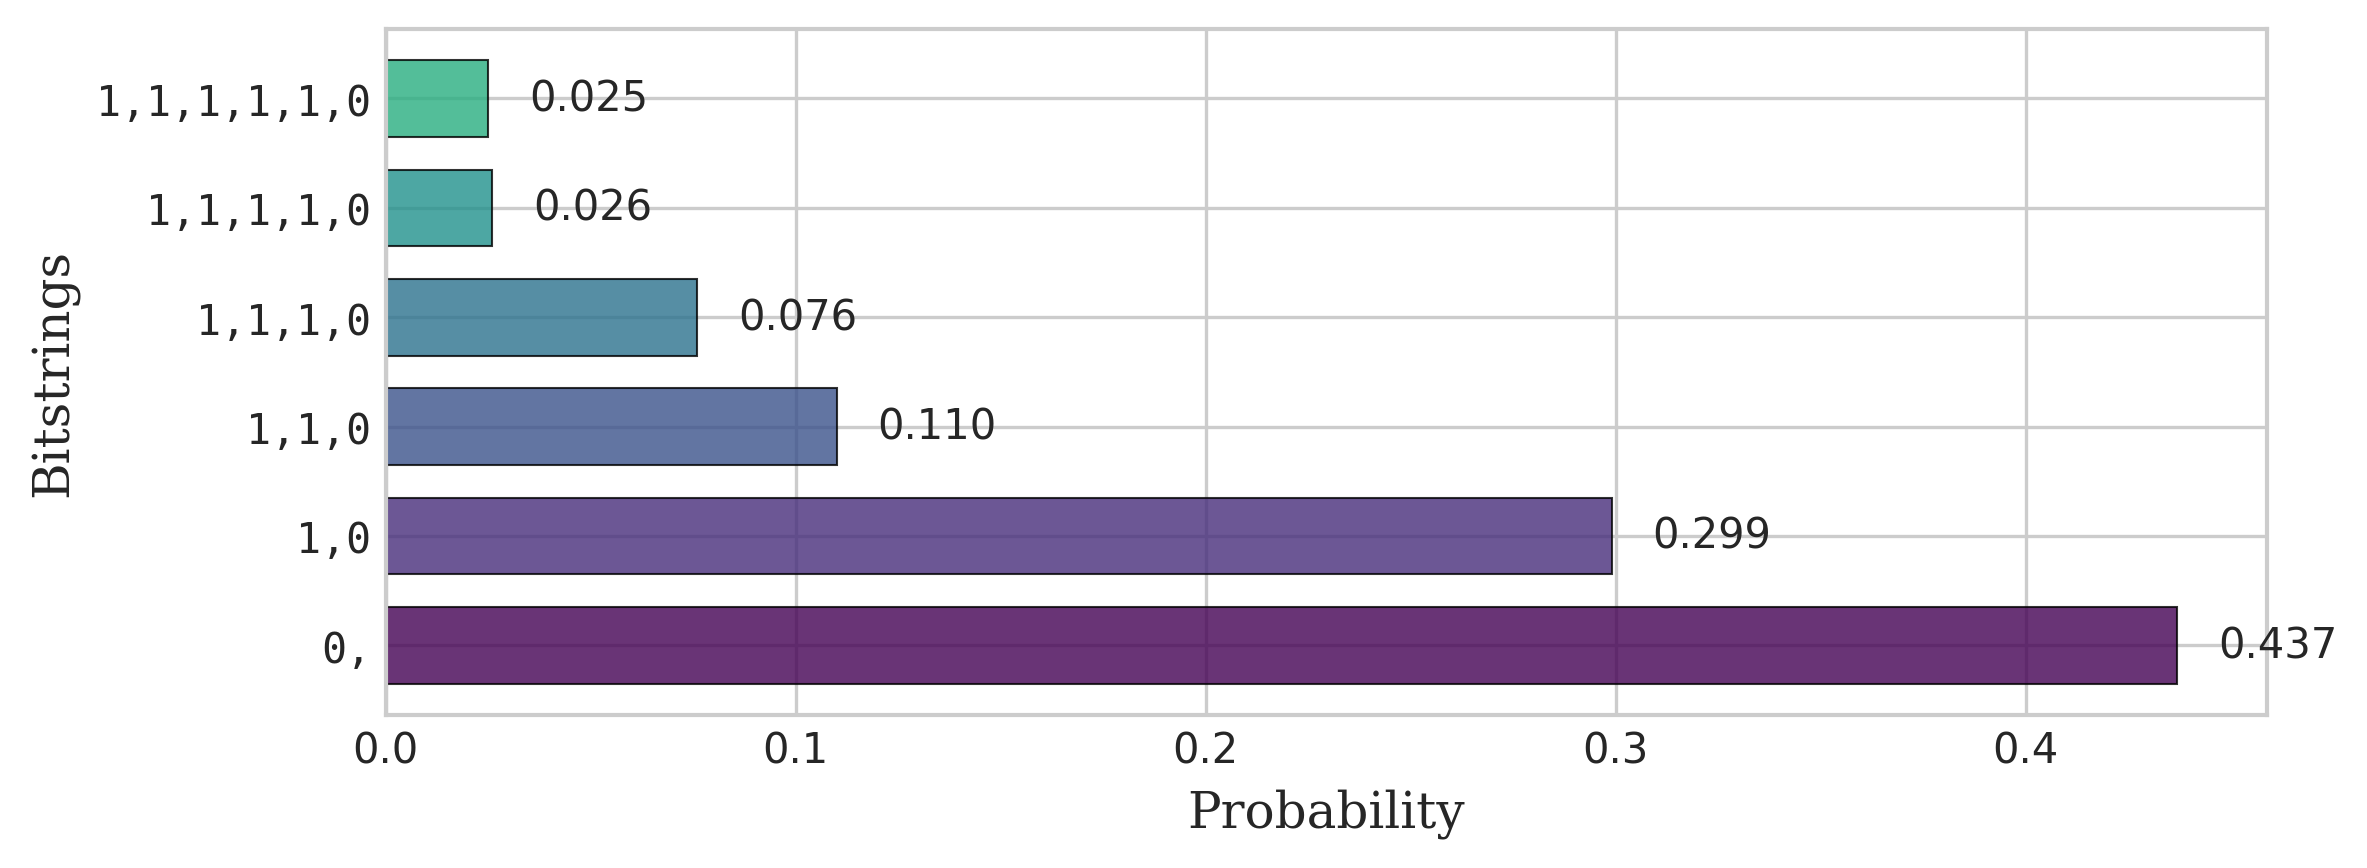
\includegraphics[width=\textwidth]{figures/repeat_until_success_simple.png}
\end{minipage}
\hfill
\begin{minipage}{0.48\textwidth}
\centering
\scriptsize
\begin{tabular}{|r|c|c|}
\hline
Bitstring & Probability & Expected Formula \\
\hline
0, & 0.4700 & $1/2^{1}$ \\
1,0 & 0.2720 & $1/2^{2}$ \\
1,1,0 & 0.1400 & $1/2^{3}$ \\
1,1,1,0 & 0.0580 & $1/2^{4}$ \\
1,1,1,1,0 & 0.0190 & $1/2^{5}$ \\
1,1,1,1,1,0 & 0.0180 & $1/2^{6}$ \\
1,1,1,1,1,1,0 & 0.0160 & $1/2^{7}$ \\
\hline
\end{tabular}
\end{minipage}
\caption{Results from the repeat-until-zero program simulated using qstack. The histogram (left) shows the distribution of measurement outcomes resulting from 1000 simulation runs, where each bitstring represents a sequence ending in successful termination (0). The table (right) compares the observed probabilities against theoretical expectations. The close agreement validates the qstack implementation.}
\label{fig:repeat-until-success}
\end{figure}

Beyond demonstrating probabilistic quantum behavior, this example illustrates qstack's core programming pattern. Programs in qstack follow an allocate/compute/measure/callback structure: quantum resources are allocated in a nested fashion, quantum operations are performed within these allocation scopes, measurements are taken at specific points, and classical callbacks process measurement results to determine whether additional quantum computation should be generated. This pattern naturally supports the iterative and conditional execution common in quantum algorithms, particularly those requiring error correction or probabilistic success patterns. This pattern is a generalization of, and can trivially support, a static model where all qubits are allocated at once and measured at a computation's end.

%This example also demonstrates qstack's key design principle: inversion of control where quantum execution is primary, while %classical computation occurs via callbacks that can dynamically generate new quantum instructions based on measurement outcomes.

Later examples show the true expressiveness of qstack by having measurements observe only part of a quantum state, preserving entanglement and superposition for other parts of the state while still observing enough to effect dynamic adjustments such as error correction. We present no new algorithms, but rather a programming framework well-aligned to expressing existing algorithms in natural ways that compose.

Our model introduces these key innovations:

\begin{enumerate}
\item \textbf{Stack-based qubit allocation}: Rather than preallocating a fixed qubit set, qubits are allocated and measured in a nested fashion, with each measurement applying to the most recently allocated qubit. Measurement results are passed to arbitrary classical functions. This approach enables dynamic resource management and simplifies the implementation of complex quantum algorithms with varying qubit requirements.

\item \textbf{Callback-based classical logic}: When classical logic is required during quantum execution, it is introduced via callbacks, classical computations that determine whether additional quantum instructions should be incorporated based on measurement results. This provides direct support for iteration at each level of nested qubit allocation.

\item \textbf{Modular execution}: This structure promotes modularity, allowing classical computations to be interleaved with quantum code even when those classical operations trigger additional quantum subcomputations. This modularity is particularly important for implementing error correction protocols, where syndrome measurements trigger appropriate quantum correction operations. What might be a pure quantum computation at a higher level of abstraction becomes a hybrid computation after translation to a lower level without any need to violate abstractions or reason globally.
\end{enumerate}

Our approach focuses on providing a programming framework that supports various instruction sets rather than prescribing a specific universal set. Programs written in qstack can target different hardware platforms through their respective instruction sets. This flexibility allows quantum computations to be described at different layers of abstraction, accommodating both hardware-specific constraints and algorithm-level optimizations within the qstack programming model. 

The remainder of this paper presents qstack's key aspects via examples and programming patterns (Section~\ref{sec:examples}), instruction generation (Section~\ref{sec:synthesis}), callback mechanisms (Section~\ref{sec:callbacks}), formal semantics (Section~\ref{sec:formal}), error correction (Section~\ref{sec:error-correction}), implementation details (Section~\ref{sec:implementation}), evaluation against other frameworks (Section~\ref{sec:evaluation}), related work (Section~\ref{sec:related}), and future directions (Section~\ref{sec:conclusion}).
